\documentclass{article}

% Packages for setting up page margins
\usepackage[margin=1in]{geometry}

\usepackage{graphicx, setspace, amsmath, mathtools, amssymb, url, float}
\setlength{\parskip}{2mm}
\graphicspath{ {./images/} }

% Title
\title{CS535 Design and Analysis of Algorithms - Assignment 2}
\author{Batkhishig Dulamsurankhor - A20543498}
\date{\today} % Use \date{} for no date

\begin{document}

\maketitle

\begin{enumerate}
  \item
  \begin{enumerate}
    \item In this problem, I am making assumption that the number of nodes in $k$ heaps has to be a power of two. 
    If the total number is not power of two, then we cannot end up with one heap as described in the question.
    \begin{enumerate}
      \item If we perform serial merge on $k$ number of Binomial heaps, it will perform very well when the tree ranks are fairly different from one another.
      Let's say rank of a tree is $r_k$ for the $kth$ tree. For example, we have two trees of $r_4$ and one tree of $r_5$ and one tree of $r_6$ and another tree of $r_7$.
      Then merging serially would be quite simple, we just merge the first two trees, then we have two $r_5$ trees and merge them as well, and so on. We will eventually left with $r_8$ tree.
      However, if we have a forest with the same rank trees, the serial merge wouldn't work well.
      Cause we merge the first two trees and we will try to merge them with the rest of the trees, which is costly cause there is none with the same rank and we will have to check the forest exhaustively.
      We can only merge the tree when a new tree with the same rank is created finally.
      After each iteration, we still have to go through the whole Binomial heaps and if we assume that each merge between two trees takes constant time, the total time complexity of the algorithm is $O(k^2)$.
      \item For binary merge, we have the number trees potentially halved after each iteration.
      However, we still have to go through each trees when have a case similar to the first example when we had the trees with fairly different ranks from one another.
      The time complexity of this algorithm will be $O(klogk)$ since the number of trees can be halved on each iteration.
    \end{enumerate}
    \item One important property of Binamial heap is that the number of nodes in a tree will always be power of $2$.
    For example, the tree with rank $r=3$ has $8$ number of nodes and merging two trees with this rank results in a new tree with rank $r=4$ and $16$ nodes in total.
    Let's represent the number of nodes of the trees in binary number: $N_3=8=2^3=1000_2$ and $N_4=16=2^4=10000_2$.
    If we look closely, we can see that after one merge the two trees with $01000_2$ (added leading 0 to show the flip) rank produces a tree with rank $10000_2$ and we did exactly one bit-flip.
    This is true for every merge, since the number of nodes in a binary tree is always power of $2$.
    So merging the k heaps serially results in the number of merge being equal to the number of bit-flips. 
  \end{enumerate}

  \item The rank of a Fibonacci heap is lower bounded by $O(log_2n)$ where $n$ is the number of nodes, because the heap that has not been cut yet been cut is basically a Binomial heap. In other words, no decrease key operation has been executed on the heap.
  The upper bound of the rank would be $O(log_{\phi}n)$, the reason is that in a Fibonacci heap, the minimum possible number of node a heap can have is a number that has a golden ratio where highest possible grandchildren of the root node has been cut.
  
  In Fibonacci heaps, we do not have One Rank Rule like in Binomial heap. However, if we were to minimize the number of nodes in the
  heap, we must have the higher rank tree to be built with the minimum number of nodes for the lower rank tree. That way we can end up with the fewest possible nodes.
  Let's say we have $k$ number of trees, meaning the rank of the biggest tree is $k$. Let's start the recurrence with the first few trees.

  \begin{figure}[H]
    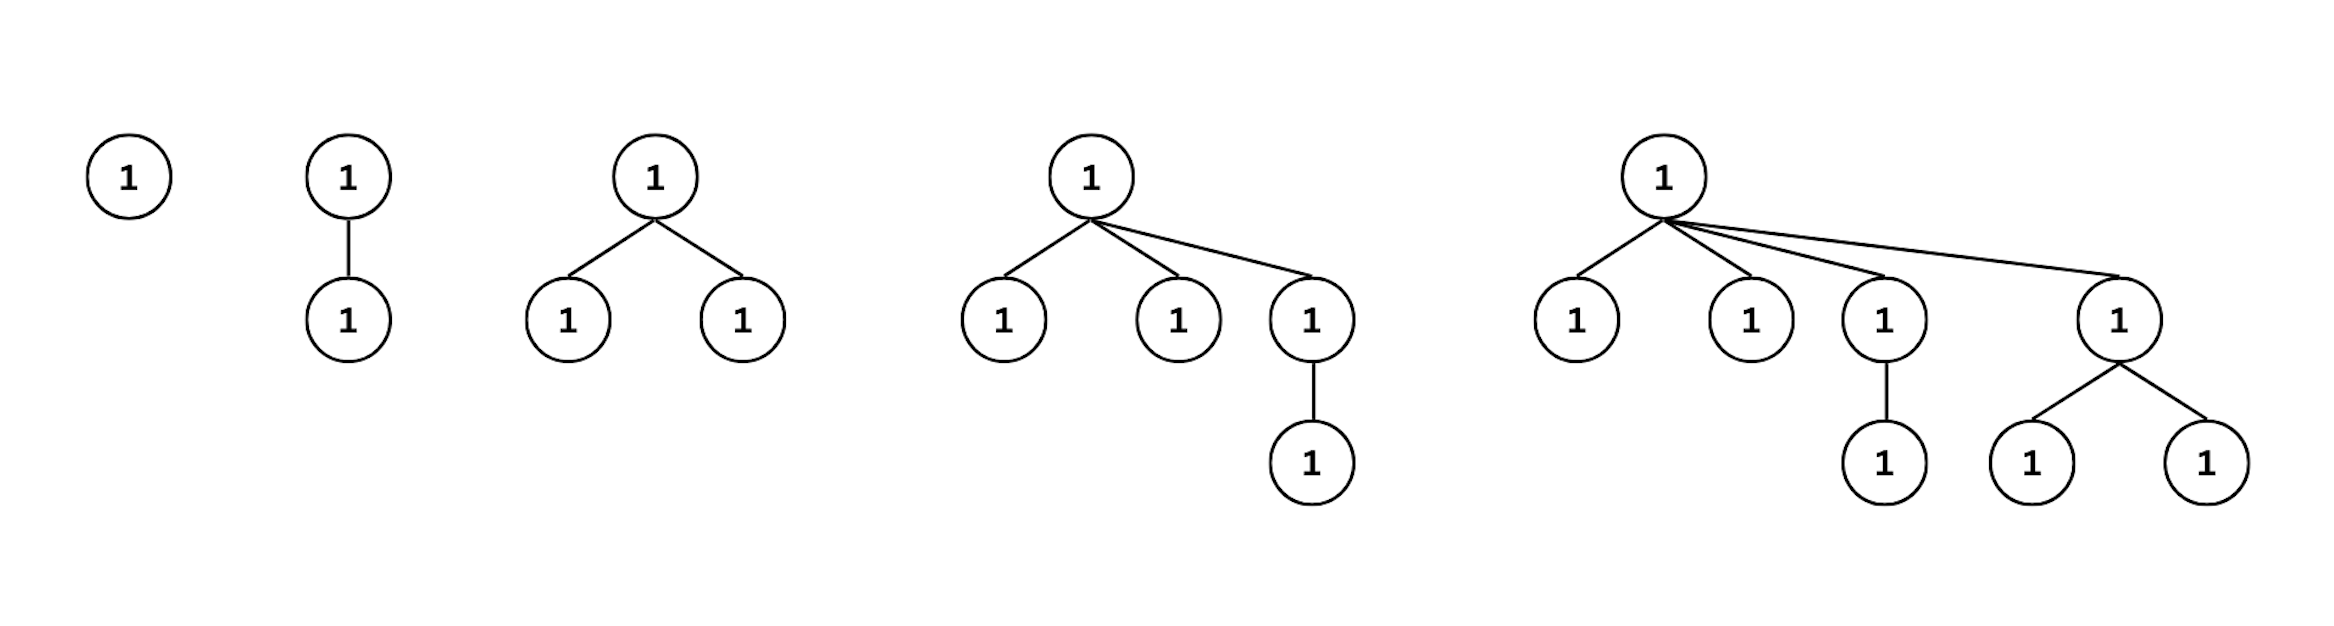
\includegraphics[width=\textwidth]{image1.png}
    \caption{Disclaimer: Each tree has a valid heap structure (not 1s)}
    \centering
  \end{figure}

  If we look closely, $r=2$ tree is made up of $r=0$ and $r=1$ trees, $r=3$ tree is made up of $r=2$ and $r=1$ trees and on and on.
  In other words, the number of nodes at $N_k=N_{k-1}+N_{k-2}$, which is a Fibonacci sequence.

  $N_2=N_1+N_0$

  $N_3=N_2+N_1$
  
  $...$

  $N_k=N_{k-1}+N_{k-2}$

  Solving the recurrence results in $N_k=\phi^r$.\cite{master}.
  
  So the minimum number of nodes in a Fibonacci heap has becomes the following according to the Fibonacci sequence expression\cite{wiki}:
  
  $N_k=((1+\sqrt(5))^k-(1-\sqrt(5))^k)/\sqrt(5).$

  \item As we have discussed on the previous problem, we need to be left with only one tree that is made up with the previous two trees.
  $N_k=N_{k-1}+N_{k-2}$. The tree is left with subtrees of all the previous ranks that are marked, decrease key has been executed
  once for each of them.

  Also, we can create such tree by executing a sequence of decrease key operations on a non-cut tree. We can decrease key for nodes that are lower or equal level than the grandchildren of the root node.
  Plus, they must have the most number of nodes among their siblings and none of their sibling must have been cut. If so, their parent must be cut and the total rank of the heap might decrease.
  Let's say we had the following tree.
  \begin{figure}[H]
    \centering
    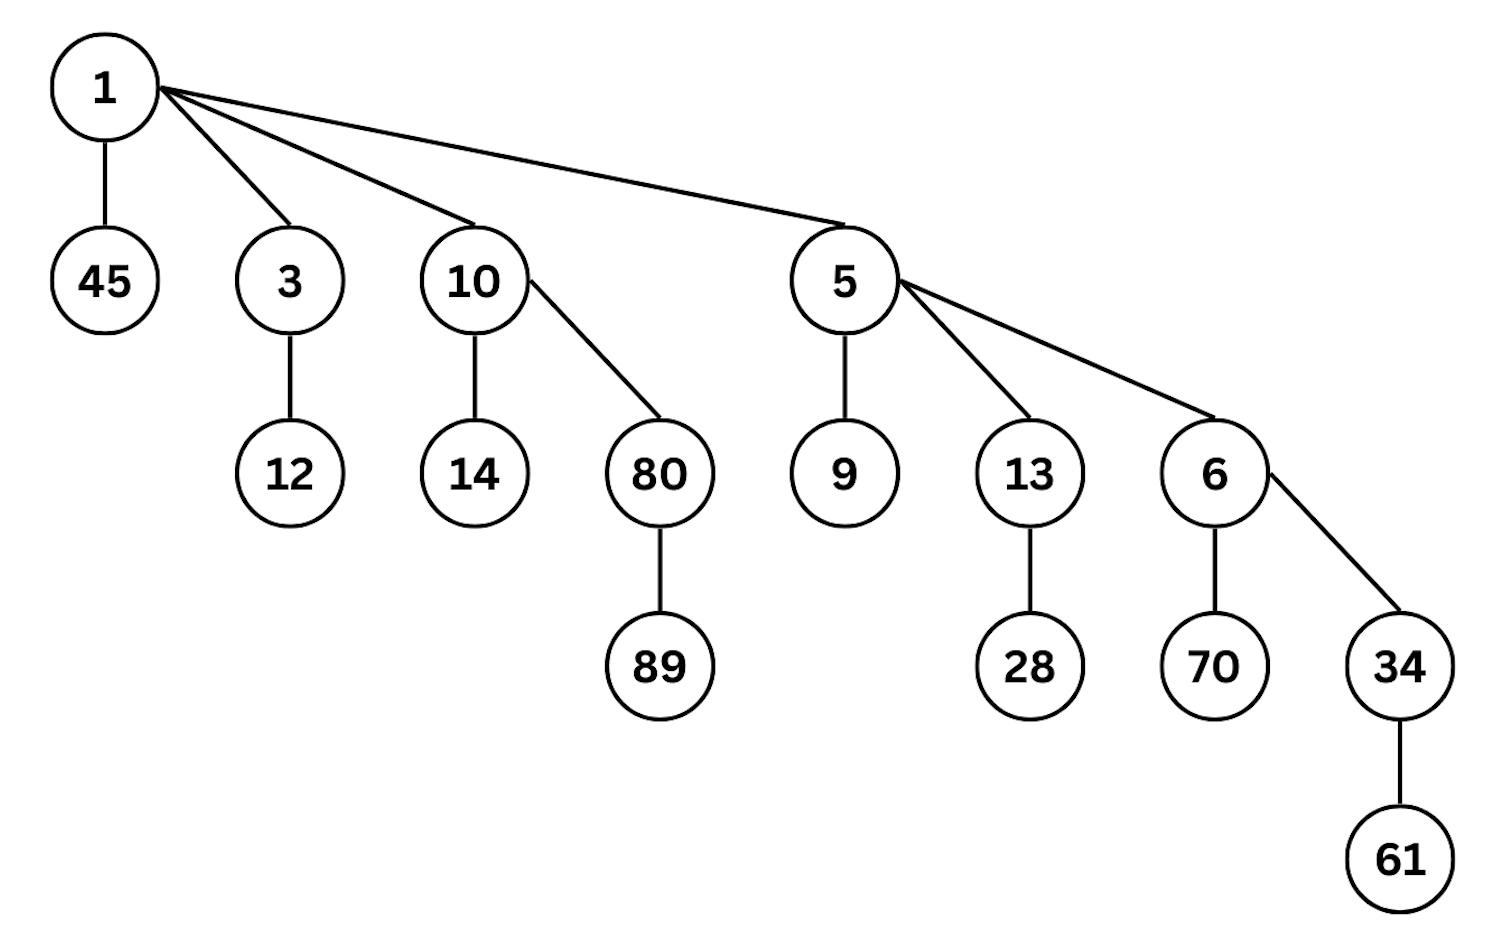
\includegraphics[width=0.5\textwidth]{image3.png}
    \caption{Initial heap with Binomial heap structure.}
  \end{figure}

  We run the following sequences of decrease key:

  $decrease\_key(6);$

  $decrease\_key(28);$

  $decrease\_key(80);$

  $decrease\_key(12);$

  The resulting tree will be a tree with rank $4$ with the fewest possible number of nodes, which is $8$.
  \begin{figure}[H]
    \centering
    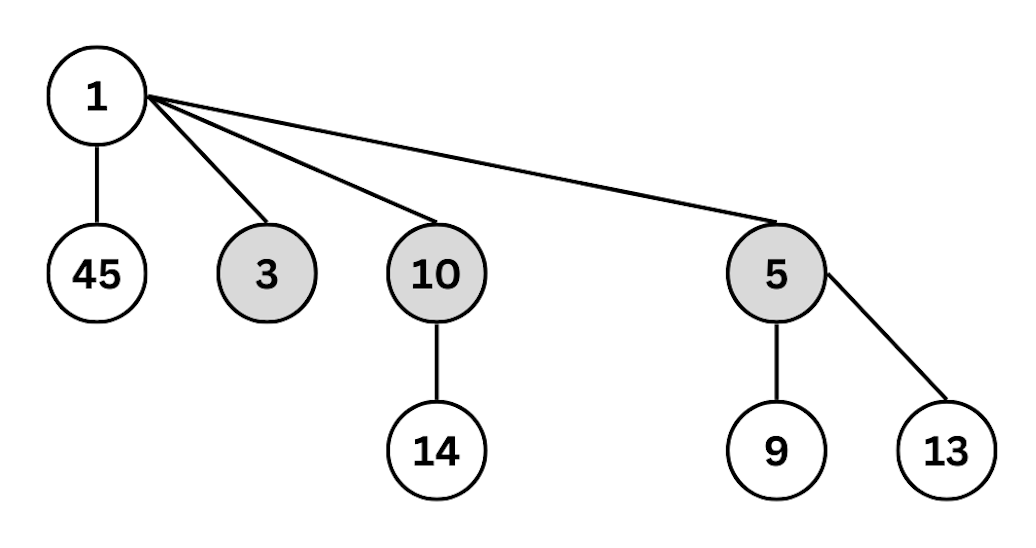
\includegraphics[width=0.5\textwidth]{image4.png}
    \caption{Resulting heap. Gray nodes are marked because one of their children has been removed.}
  \end{figure}

  \item Insertion bound stays the same for allowing $k$ children to be deleted before deleting a node.
  Since insertion doesn't involve cutting a node, the amortized cost is still $O(1)$.
  
  Allowing $k$ subtrees to be cut before cutting the node makes the algorithm lose its Fibonacci property, unless $k=1$.
  For decrease key, the time complexity is still amortized $O(1)$. Because, decreasing $n$ number of nodes will now result in maximum $n+n/k$
  number of trees which is less than Fibonacci heap's $n+n$ when $k>1$.
  
  For delete min, let's say the heap has the minimum value in a maximum rank tree $r$. When the root is removed, each of the children becomes a new root.
  It takes $O(r)=O(logn)$ to execute this step. Next, We have to merge the trees with the same rank.
  However, we can potentially have many trees with the same rank depending on $k$. That makes the merge operation costly compared to Fibonacci's heap.
  The cost for merging step is $O(logn+k)$.
  And finally, we have update the minimum pointer which takes $O(logn)$. Overall, the running complexity is bounded by $O(logn+k)$.
  
  The recurrence is similar to Fibonacci sequence but the minimum number of nodes in a tree is can be more as $k$ increases, specifically a sum of previous $k+1$ heaps.
  Cause we are more likely to keep more nodes before cascading cutting the parent as $k$ increases.

  $N_r=N_{r-k-1}+N_{r-k-2}+...+N_{r-1}$

  When $k=1$, we should have a Fibonacci sequence, which is true:

  $N_r=N_{r-2}+N_{r-1}$

  \item
  \begin{enumerate}
    \item Union-find
    \begin{figure}[H]
      \centering
      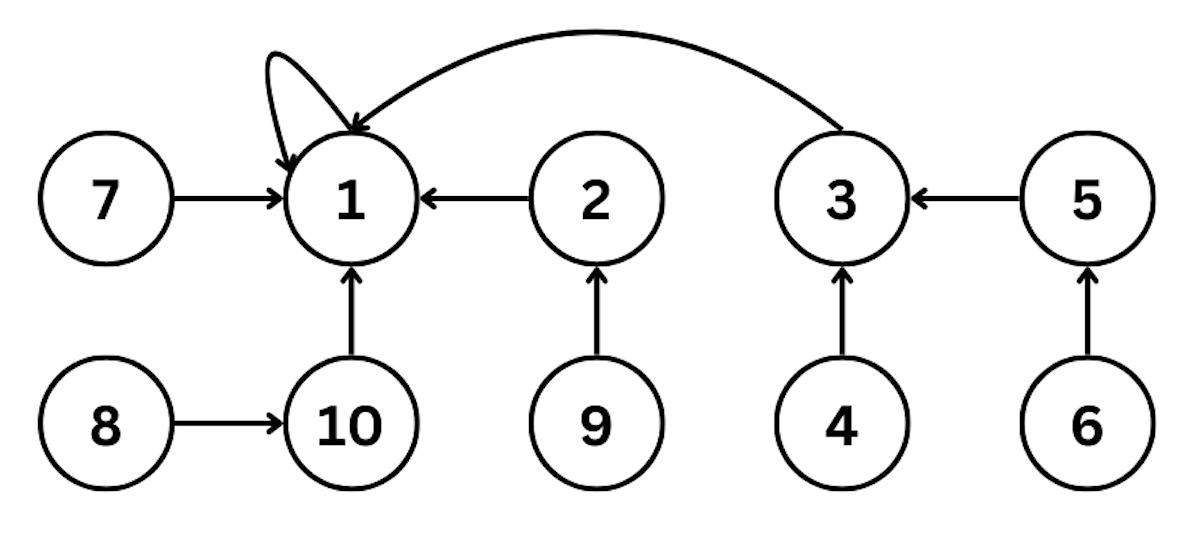
\includegraphics[width=0.5\textwidth]{image2.png}
      \caption{Resulting tree without path compression.}
    \end{figure}
    \item Partial FIND needs to goes up to the node which was the root of the set when the FIND operation took place.\cite{master}

    \begin{enumerate}
      \item $F(9)$.

      \begin{figure}[H]
        \centering
        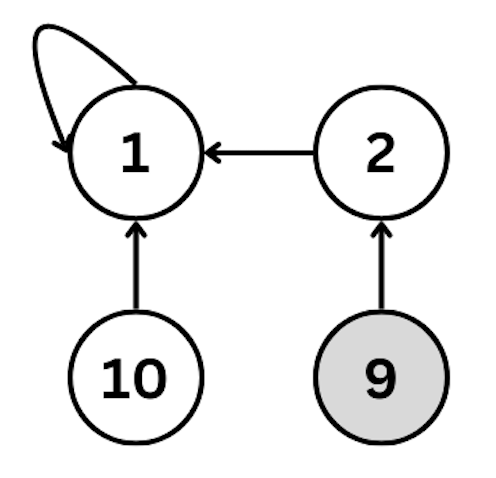
\includegraphics[width=0.2\textwidth]{image5.png}
        \caption{$F(9)$ operation returns root node $1$.}
      \end{figure}

      \item $F(6)$.

      \begin{figure}[H]
        \centering
        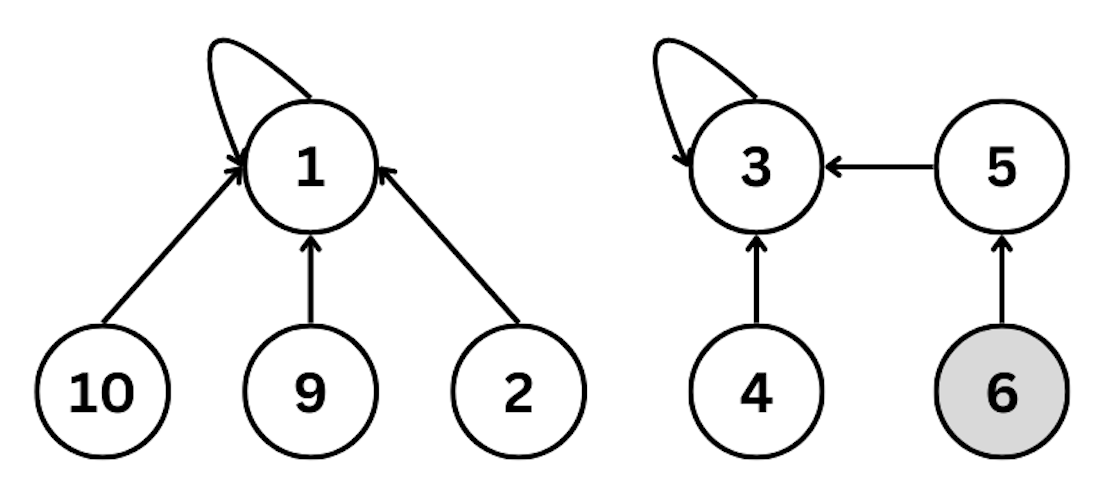
\includegraphics[width=0.5\textwidth]{image6.png}
        \caption{$F(6)$ operation returns root node $3$.}
      \end{figure}

      \item $F(4)$.

      \begin{figure}[H]
        \centering
        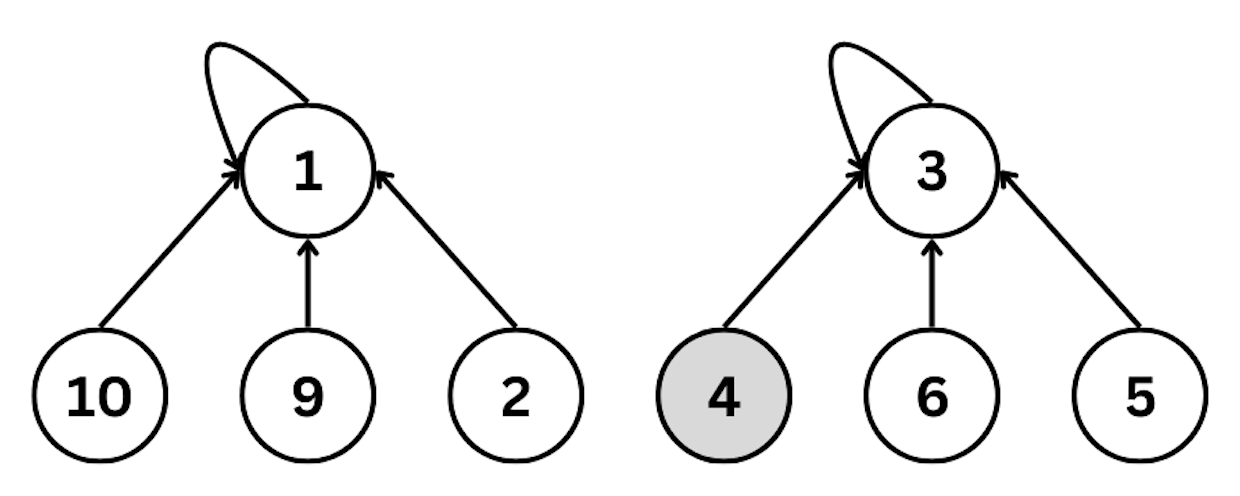
\includegraphics[width=0.5\textwidth]{image7.png}
        \caption{$F(4)$operation returns root node $3$.}
      \end{figure}

      \item $F(8)$.

      \begin{figure}[H]
        \centering
        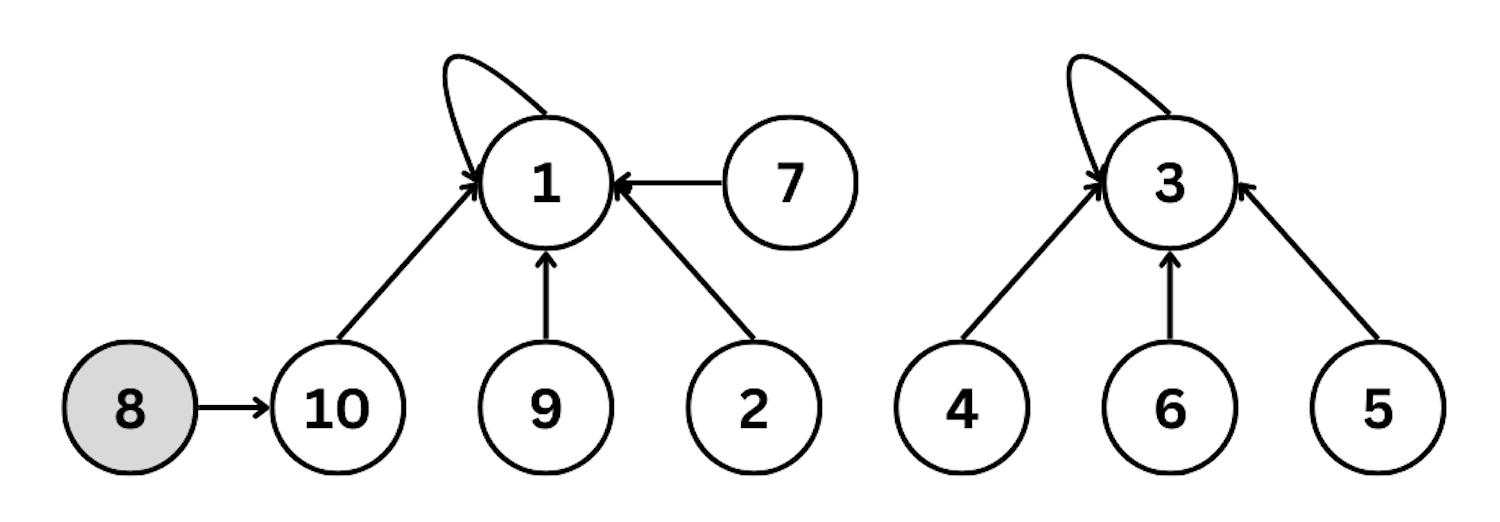
\includegraphics[width=0.5\textwidth]{image8.png}
        \caption{$F(8)$ operation returns root node $1$.}
      \end{figure}

      \item $F(5)$.

      \begin{figure}[H]
        \centering
        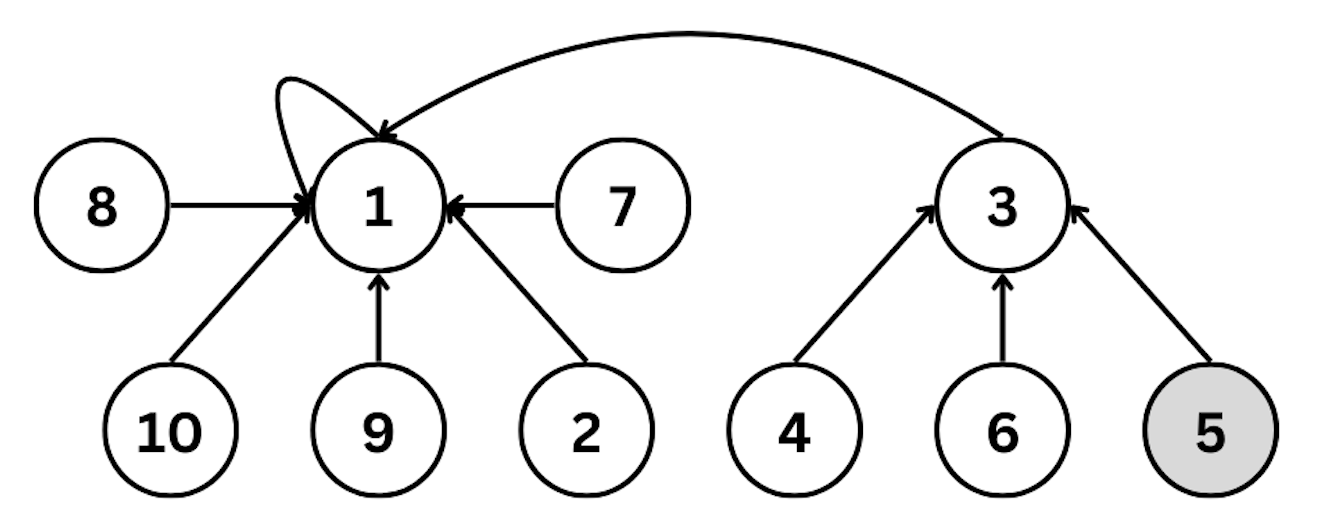
\includegraphics[width=0.5\textwidth]{image9.png}
        \caption{$F(5)$ operation returns root node $1$.}
      \end{figure}

      \item $F(7)$.

      \begin{figure}[H]
        \centering
        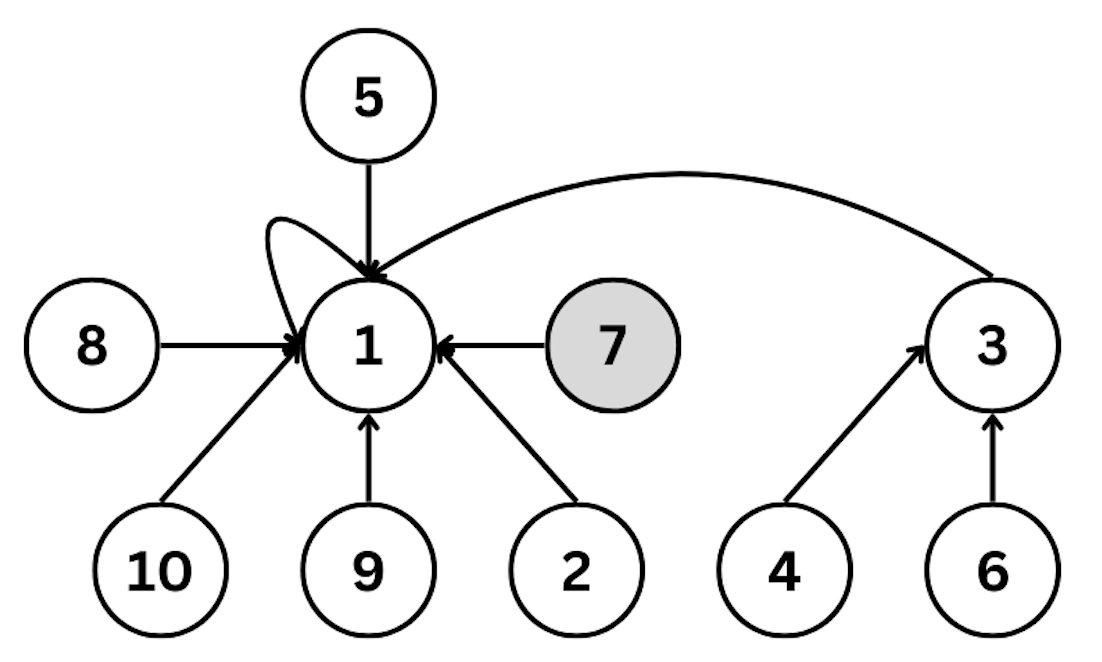
\includegraphics[width=0.4\textwidth]{image10.png}
        \caption{$F(7)$ operation returns root node $1$.}
      \end{figure}

    \end{enumerate}
    \item In general, without path compression, union find requires $O(n)$ in worst case, where $n$ is number of items.
    The worst case is when the tree's height is $n$ (like linked list), and finding the root of leaf takes $O(n)$ times.

    With path compression the time complexity of union-find is amortized constant time.

    For above example:
    \begin{enumerate}
      \item $F(9)$. Without compression it is $O(2)$, cause we are just traversing up.
      With compression it is $O(3)$, we traverse and compress the path for node 9.

      \item $F(6)$. Same for $F(6)$. Without compression it is $O(2)$, cause we are just traversing up.
      With compression it is $O(3)$, we traverse and compress the path for node 6.

      \item $F(4)$. Without compression it is $O(1)$, cause it is connected to the root $3$.
      With compression it is also $O(1)$ since we don't need to compress.

      \item $F(8)$. Without compression it is $O(2)$, cause we are just traversing up.
      With compression it is $O(3)$, we traverse and compress the path for node 8.

      \item $F(5)$. Without compression it is $O(2)$, cause we are just traversing up.
      With compression it is $O(3)$, we traverse and compress the path for node 6 up to root 1.

      \item $F(7)$. Without compression it is $O(1)$, cause it is connected to the root $1$.
      With compression it is also $O(1)$ since we don't need to compress.
    \end{enumerate}
  \end{enumerate}
  \item hello

\end{enumerate}

\begin{thebibliography}{9}

\bibitem{master}
master.pdf.

\bibitem{wiki}
Fibonacci sequence, \emph{Wikipedia}, \url{https://en.wikipedia.org/wiki/Fibonacci_sequence#Relation_to_the_golden_ratio}

\end{thebibliography}


\end{document}